\documentclass{article}
\usepackage{graphicx}
\usepackage{float}
\usepackage{subcaption}
\usepackage{amsmath}
\usepackage[colorlinks=true, allcolors=blue]{hyperref}

\bibliographystyle{alpha}

\title{Information Theory \\ \large Problem Set 05 - Stream Codes}
\author{Luís Felipe Ramos Ferreira}
\date{\href{mailto:lframos\_ferreira@outlook.com}{\texttt{lframos\_ferreira@outlook.com}}
}

\begin{document}

\maketitle

\begin{enumerate}
	\item \begin{enumerate}
		      \item Handmade exercise.
		            \begin{figure}[H]
			            \centering
			            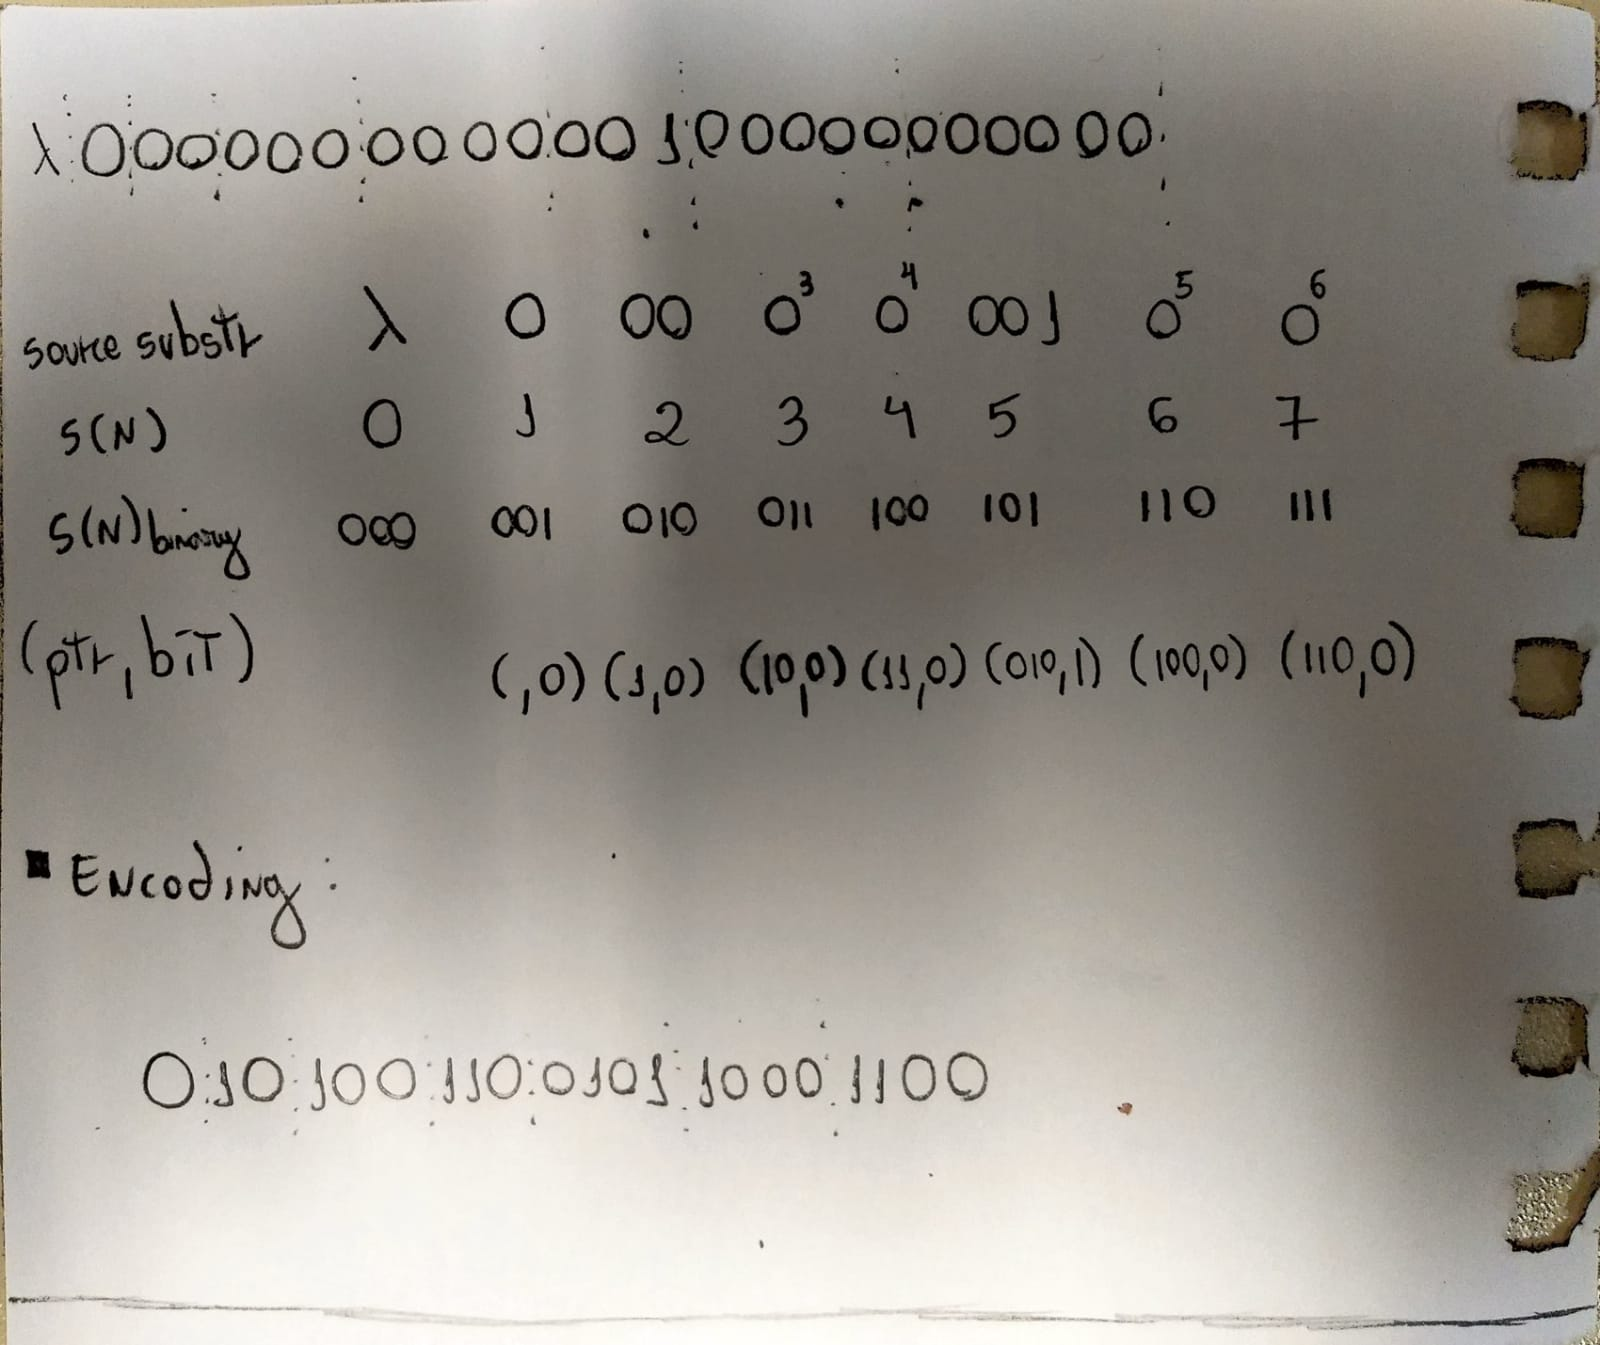
\includegraphics[width=0.8\textwidth]{images/5-1-a.jpeg}
		            \end{figure}

		      \item Handmade exercise.
		            \begin{figure}[H]
			            \centering
			            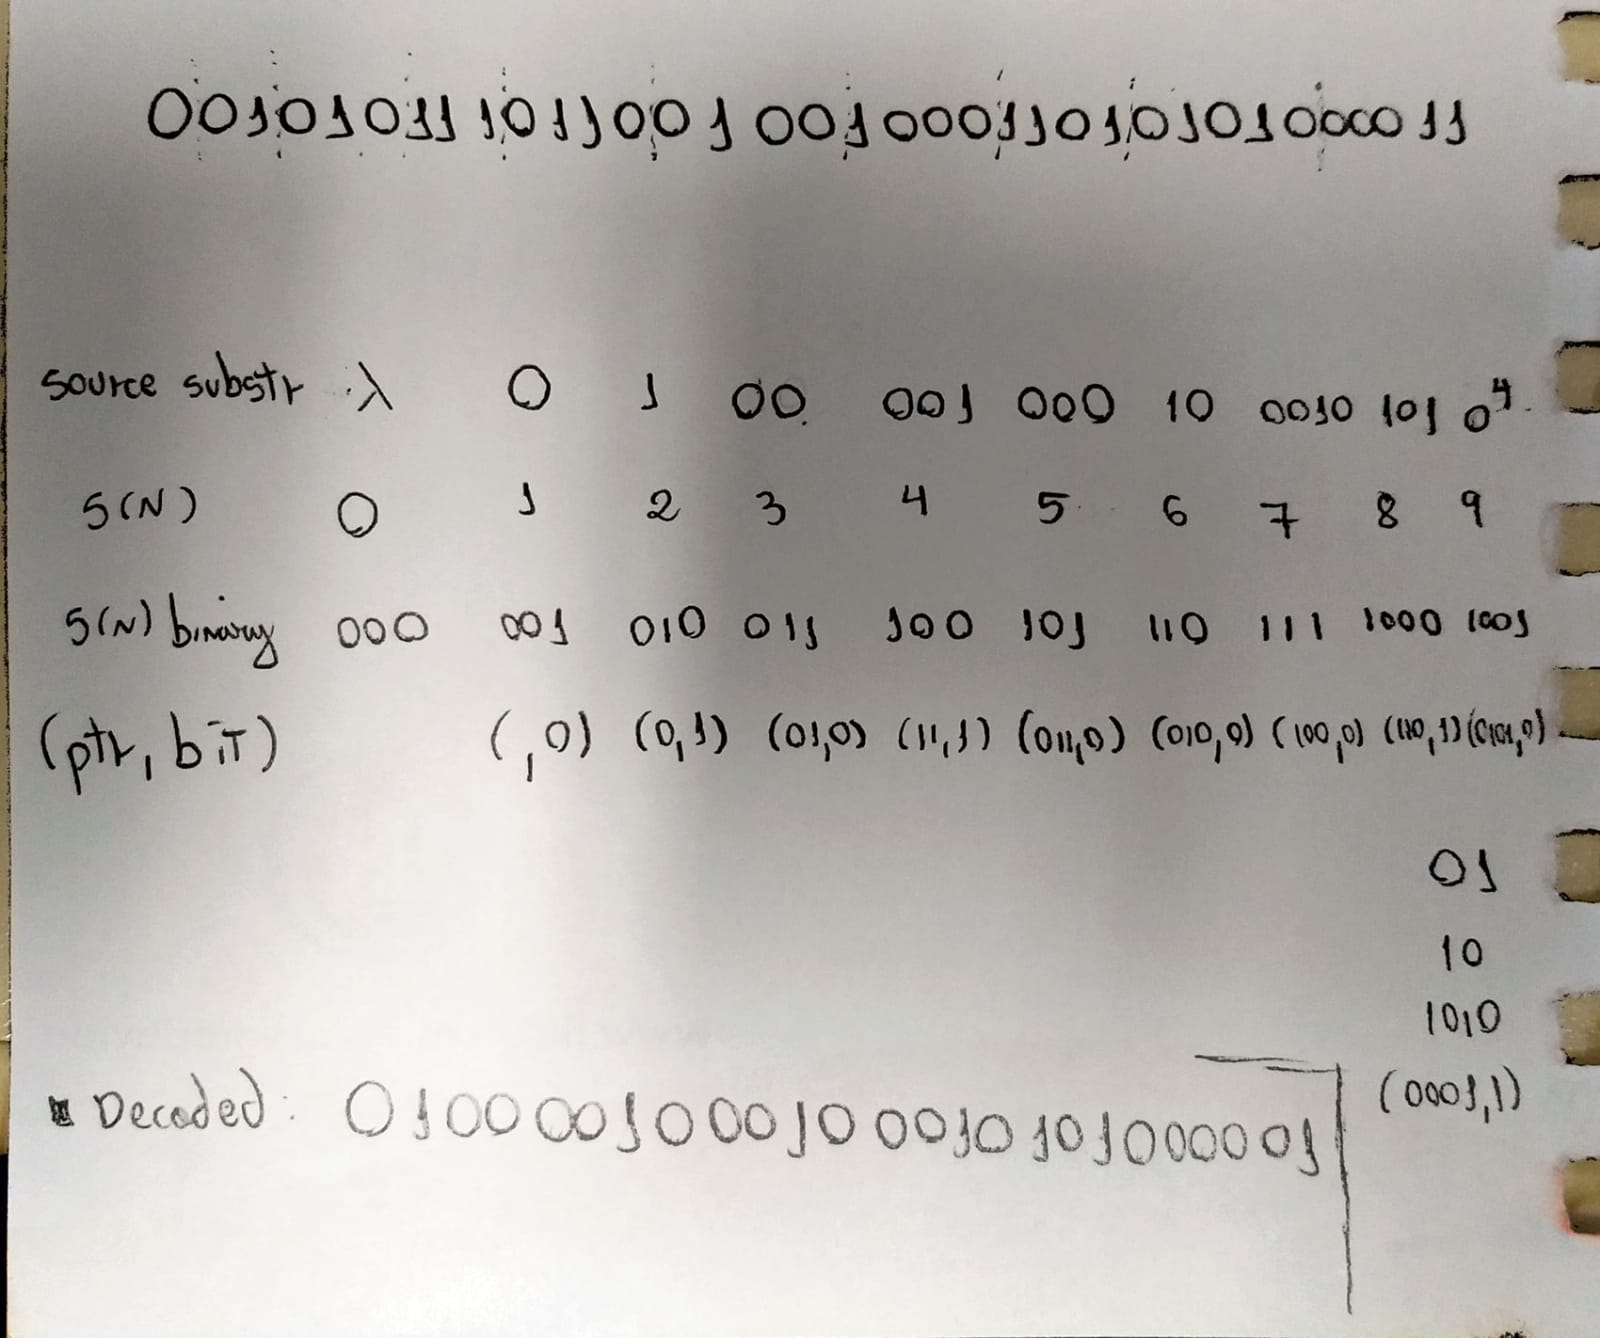
\includegraphics[width=0.8\textwidth]{images/5-1-b.jpeg}
		            \end{figure}
	      \end{enumerate}
	\item \begin{enumerate}
		      \item The three claims from the student are correct. Claims 1 and 2 are true because they basically follow the property stated by the Source Coding Theorem for symbol codes. Claim 3 is true because of a transitive property. Since each symbol in \(X\) is represented in \(Y\) by aproximately \(H(X)\) bits and each symbol in \(Y\) is represente din \(Z\) by aproximately \(H(Y)\), then each symbol in \(X\) is represented in \(Z\) by aproximately \(H(X) H(Y)\) bits.
		      \item \(Z\) cannot be smaller than \(Y\), because of the source coding theorem. Otherwise, we would have a compression algorithm better than the theoretical limit, i.e., we would have a compresison algorithm that compress the file using less than \(H(X)\) bits per symbol of the original file. So \(Y\) and \(Z\) must have aproximately the same size.
		      \item Since \(Z\) uses aproximately \(H(X) H(Y)\) bits per source symbol and \(Y\) uses aproximately \(H(X)\) per source symbol, we have that \(H(X) H(Y) = H(X)\), because of what was discussed in the previous section. So, we have that \(H(Y)\) is aproximately 1.
		      \item Since \(H(Y)\) is aproximately 1 per bit, we can say that the proportion of 1's and 0's in a optimally compressed file is uniform or almost uniform. That's the whole point of the compression, removing the redundancy from the original file and achieving the smallest file posible without loosing information.
	      \end{enumerate}
\end{enumerate}
\end{document}
